%       $Id$    
\documentclass{article}

\usepackage{listings}
\usepackage[T1]{fontenc}
\usepackage[scaled=0.8]{luximono}
\usepackage[scaled=0.9]{helvet}
\usepackage{mathptmx}
\usepackage{xspace}
\usepackage{color}
\usepackage{graphicx}
\usepackage{psfrag}
\usepackage[landscape,a4paper,margin=1cm,dvips]{geometry}
\usepackage{multicol}
%\renewcommand{\ttdefault}{0t6c}

\newcommand{\PPthree}{\textsf{PP3}\xspace}

\lstdefinestyle{pp3}{morecomment=[l]\#,numbers=none,numberstyle=\sffamily\scriptsize,
  keywords={filename,set,color,switch,on,off,penalty,objects\_and\_labels,delete,
    add,reposition,delete_labels,add_labels,set_label_text,text,at,along,towards,tics,
  line_width,line_style,penalties},
  basicstyle=\ttfamily, fontadjust, string=[b]{"},
  stringstyle=\texttt,aboveskip=0pt,belowskip=-\medskipamount,escapeinside=`'
                                ,backgroundcolor=\color[gray]{0.9}
}

\lstdefinestyle{shell}{numbers=none,numberstyle=\sffamily\scriptsize,
  basicstyle=\ttfamily, fontadjust, columns=[l]fullflexible,
  stringstyle=\texttt,aboveskip=0pt,belowskip=-\medskipamount,escapeinside=`',backgroundcolor={}}

\lstset{style=pp3}

\parindent0pt
\parskip\medskipamount
\newskip\subsubskipamount\subsubskipamount\bigskipamount
\newskip\subskipamount\subskipamount1.5\subsubskipamount
\newcommand{\subskip}{\bigskip\medskip}
\newcommand{\subsubskip}{\bigskip}

\setcounter{secnumdepth}{-2}

\raggedbottom\raggedcolumns
\begin{document}\raggedright\small\setlength{\columnsep}{2cm}
\pagestyle{empty}

\begin{multicols*}{3}
\title{\PPthree reference card}
\author{\texttt{http://pp3.sourceforge.net}}
\date{for version 1.3}
  \maketitle\thispagestyle{empty}

%% \section{Invocation}

%% The calling syntax is very simple:
%% \begin{lstlisting}[style=shell]
%%   pp3 `\textit{<input-script-filename>}'
%% \end{lstlisting}
%% If you substitute ``\verb|-|'' for
%% ``\textit{\texttt{<input-script-filename>}}'' then \PPthree reads the input
%% from stdin.

%% The output is written to the file given in the input script, or to stdout.

%% In the following, the input script format is described.

\section{General structure}

\begin{lstlisting}
# Some introductory comments,
# i.e. what the file is about to do.

`\textrm{[Section I: Parameters.]}'

objects_and_labels

`\textrm{[Section II: Delete/add/modify objects and/or labels]}'
\end{lstlisting}
Both sections may be empty.  If section~II is empty,
\lstinline{objects_and_labels} should be omitted.

\section{Section I: Parameters}

The following top level keywords are allowed here: \lstinline{filename},
\lstinline{set}, \lstinline{switch}, \lstinline{color}, \lstinline{line_width},
\lstinline{line_style}, and \lstinline{penalties}\footnote{not explained on
  this reference card}.\subskip

\begin{lstlisting}
filename output orion.tex
\end{lstlisting}
writes the result to the file \verb|orion.tex|.  The file extension must be
\verb|.tex| and must not be omitted.\subsubskip

\begin{lstlisting}
filename stars               stars.dat
filename nebulae             nebulae.dat
filename label_dimensions    labeldimens.dat
filename constellation_lines lines.dat
filename boundaries          boundaries.dat
filename milky_way           milkyway.dat
\end{lstlisting}
This lets \PPthree look for the respective data in the given file.  The
filenames must be full paths from the current directory.\subsubskip

\columnbreak
\begin{lstlisting}
filename latex_preamble mypreamble.tex
\end{lstlisting}
makes \PPthree include the file \verb|mypreamble.tex| with e.\,g.\ font
parameters in every \LaTeX\ run.\subsubskip

\begin{lstlisting}
filename include myproject.pp3
\end{lstlisting}
includes \verb|myproject.pp3| that itself has a normal input script structure,
except for the limitation that it mustn't include yet another file.\subskip

\begin{lstlisting}
set center_rectascension  5.8
set center_declination    0
\end{lstlisting}
This sets the center of the printed map to the celestial coordinates
$(5^{\mathrm h}48',0^\circ)$.\subsubskip

\begin{lstlisting}
set box_width  15
set box_height 15
\end{lstlisting}
sets the dimensions of the printed map in centimetres.  (15~for both is the
default.)\subsubskip

\begin{lstlisting}
set grad_per_cm 4
\end{lstlisting}
sets the scale of the map in degrees per centimetre.  (4~is the default.)\subsubskip

\begin{lstlisting}
set constellation ORI
\end{lstlisting}
tells \PPthree to highlight the boundaries of constellation Orion.  Must be in
uppercase.\subsubskip

\begin{lstlisting}
set shortest_constellation_line 0.1
\end{lstlisting}
makes \PPthree suppress all constellation lines that are shorter than
0.1~centimetres.  (This is the default.)\subsubskip

\begin{lstlisting}
set label_skip 0.06
\end{lstlisting}
sets the distance between the outer rim of the celestial object and its label
to 0.06~centimetres.  (This is the default.)\subsubskip

\begin{lstlisting}
set minimal_nebula_radius 0.1
\end{lstlisting}
means that all nebulae that would be smaller than 0.1~centimetres (in radius)
are printed with a radius of \emph{exactly} 0.1~cm.  (This is the
default.)\subsubskip

\begin{lstlisting}
set faintest_cluster_magnitude 4.0
\end{lstlisting}
suppresses by default all stellar clusters that are fainter than $4.0^{\mathrm
  m}$.  (This is the default.)\subsubskip

\columnbreak
\begin{lstlisting}
set faintest_diffuse_nebula_magnitude 8.0
\end{lstlisting}
suppresses by default all emission and reflection nebulae and all galaxies that
are fainter than $8.0^{\mathrm m}$.  (This is the default.)\subsubskip

\begin{lstlisting}
set faintest_star_magnitude 7.0
\end{lstlisting}
suppresses by default all stars and all galaxies that are fainter than
$7.0^{\mathrm m}$.  (This is the default.)\subsubskip

\begin{lstlisting}
set faintest_star_with_label_magnitude 3.7
\end{lstlisting}
means that for stars as bright as $3.7^{\mathrm m}$ or brighter get
automatically generated labels.  (This is the default.)\subsubskip

\begin{lstlisting}
set faintest_star_disk_magnitude 4.5
\end{lstlisting}
means that all stars that are fainter than $4.5^{\mathrm m}$ are printed as
mere dots instead of small circles.  (This is the default.)\subsubskip


\begin{lstlisting}
set minimal_star_radius 0.015
\end{lstlisting}
This sets the radius of the dots for all stars fainter than the limit
determined by \lstinline{faintest_star_disk_magnitude} to
0.015~centimetres.  (This is the default.)\subsubskip

\begin{lstlisting}
set star_scaling 2.0
\end{lstlisting}
makes all star circles two times bigger than normal.  (Default
is~1.0.)\subsubskip

\begin{lstlisting}
set fontsize 12
\end{lstlisting}
sets the global font size to 12\,pt.  (Default is~10.)\subskip

\begin{lstlisting}
switch milky_way            off
switch nebulae              on
switch grid                 on
switch ecliptic             on
switch boundaries           on
switch constellation_lines  on
switch labels               on
\end{lstlisting}
This switches the display of the Milky Way off, and the nebulae, coordinate
grid, ecliptic, constellation boundaries, boundaries of the highlighted
constellation, and all labels on.  This is the default.\subsubskip

\begin{lstlisting}
switch eps_output on
switch pdf_output on
\end{lstlisting}
The first line makes \PPthree generating an EPS file from the map via a dvips
call, the second creates a PDF file additionally by calling ps2pdf.\subsubskip

\columnbreak
\begin{lstlisting}
switch colored_stars off
\end{lstlisting}
This disables \PPthree's default behaviour to try to illustrate the star's
actual colour in the map.  Instead, all stars get the same colour explicitly
defined by ``\lstinline{color stars}''.\subskip

\begin{lstlisting}
color background              0   0   0.4
color grid                    0   0.298 0.447
color ecliptic                1   0   0
color boundaries              0.5 0.5 0
color highlighted_boundaries  1   1   0
color constellation_lines     0   1   0
color milky_way               0   0   1
color nebulae                 1   1   1
\end{lstlisting}
This sets the colours of these map elements to the respective RGB colour.
The colour values range from 0 to~1.  What you see here are the default
values.\subsubskip

\begin{lstlisting}
color stars                   1   1   1
\end{lstlisting}
This sets the colour of stars to white (the default), however only if you
switch \lstinline{colored_stars} off.\subsubskip

\begin{lstlisting}
color labels                  0   1   1
\end{lstlisting}
sets the colour of all automated labels to cyan (the default).\subsubskip

\begin{lstlisting}
color text_labels             1   1   0
\end{lstlisting}
sets the colour of all user defined labels to yellow (the default).\subskip

\begin{lstlisting}
line_width grid                    0.025
line_width ecliptic                0.018
line_width boundaries              0.035
line_width highlighted_boundaries  0.035
line_width nebulae                 0.018
line_width constellation_lines     0.035
\end{lstlisting}
This sets the line widths of these map elements to the respective width in
centimetres.  What you see here are the default values.\subskip

\begin{lstlisting}
line_style grid                    solid
line_style ecliptic                dashed
line_style boundaries              dashed
line_style highlighted_boundaries  dashed
line_style nebulae                 solid
line_style constellation_lines     solid
\end{lstlisting}
This sets the line styles of these map elements to the respective style.
What you see here are the default values.%\subskip

\iffalse
\begin{lstlisting}
penalties stars                    2000
penalties labels                   2000
penalties nebulae                  2000
penalties boundaries               2000
penalties constellation_lines      2000
\end{lstlisting}
This sets the label overlap penalty for the respective map element to 2000.
(Default is~1000.)\subsubskip

\begin{lstlisting}
penalties boundaries_rim           2000
penalties constellation_lines_rim  2000
\end{lstlisting}
This sets the label \emph{rim} overlap penalty for the respective map element
to 2000.  The ``rim'' is the vicinity of the label, i.\,e. this is not the
label area itself.  (Default is~1000.)\subsubskip


\begin{lstlisting}
penalties threshold                2000
\end{lstlisting}
means that all labels for which the minimal found penalty is larger than 2000
are not printed, unless you explicitly specify otherwise in the
\lstinline{objects_and_labels} section.  (Default is~1000.)\subsubskip

\begin{lstlisting}
penalties rim                      2000
\end{lstlisting}
sets the weighting of the overlap penalties with the label rim to~2000.
(Default is~1000.)
\fi


\section{Section II: Objects and labels}

The following top level keywords are allowed here: \lstinline{add},
\lstinline{delete}, \lstinline{reposition}, \lstinline{add_labels},
\lstinline{delete_labels}, \lstinline{set_label_text}, and
\lstinline{text}.\subskip

\begin{lstlisting}
add IC 5070  NGC 7000;
\end{lstlisting}
adds the nebulae IC\,5070 and NGC\,7000 to the map with their
labels.\subsubskip

\begin{lstlisting}
delete LEO 63  HD 97605 ;
\end{lstlisting}
removes the two stars 63\,Leo and HD\,97605 from the map.\subsubskip

\begin{lstlisting}
reposition LEO 32 SE ;
\end{lstlisting}
positions the label of 32\,Leo to the lower right (\lstinline{SE}${}={}$\textbf
South \textbf East).\subsubskip

\begin{lstlisting}
add_labels M 66  LEO 24 ;
\end{lstlisting}
adds the labels of M\,66 and 24\,Leo to the map.  The positioning is still
automatic.\subsubskip

\begin{lstlisting}
delete_labels M 43 ;
\end{lstlisting}
deletes the label of the nebula M\,43 from the map, \emph{not} the nebula
itself.\subsubskip

\begin{lstlisting}
set_label_text UMA 50 "\\footnotesize Dubhe"
\end{lstlisting}
replaces the default label text for 50\,UMa with
``\verb|\footnotesize Dubhe|''.\subsubskip


\begin{lstlisting}[showstringspaces=false]
text "\\small Wolf 359\\hskip0.3em
      \\psdots[dotstyle=+,dotangle=45](0,0)"
     at 10.902 7.32
     color 0.3 0.3 0.9333 towards NW ;
\end{lstlisting}
This prints the \LaTeX\ commands between the \verb|"..."| at the celestial
point $(10^{\mathrm h}54^{\mathrm m}7.2^{\mathrm s},7.32^\circ)$, in a
grey-blue colour, and to the upper left of the point.

This graphics shows the possible values for \lstinline{reposition} and the
\lstinline{towards} option (the large dots lie exactly on the celestial
position given after the \lstinline{at} option):\\[1.5ex]
\begin{psfrags}
  \def\psftt#1 {\psfrag{#1}[c][c]{\texttt{#1}}}
  \psftt E \psftt NE \psftt N \psftt NW \psftt W \psftt SW \psftt S \psftt SE
  \psfrag{E!}[c][c]{\texttt{E\_}}
  \psfrag{W!}[c][c]{\texttt{W\_}}
  \centerline{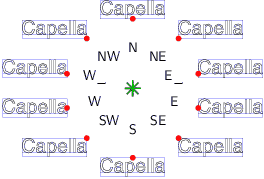
\includegraphics[scale=0.8]{pp3rose}}
\end{psfrags}\subsubskip

\begin{lstlisting}
text "$#3$" at 0 20 along declination
            tics rectascension 1 towards N ;
text "$#5$" at 11 0 along declination
            tics declination 10 towards S ;
\end{lstlisting}
This creates automatically generated labels for the $20^\circ$ declination
circle (every whole hour), and for the $11^{\mathrm h}$ rectascension line
(every 10 declination degrees).  The following placeholders are
available:\vspace{-1.5ex}
\begin{description}\itemsep-0.2ex
\item[\texttt{\mdseries \#1}] Rectascension in hours.
\item[\texttt{\mdseries \#2}] Declination in degrees.
\item[\texttt{\mdseries \#3}] Rectascension in integer hours (truncated, not
  rounded).
\item[\texttt{\mdseries \#4}] Rectascension fraction of hour in minutes
  (truncated, not rounded).
\item[\texttt{\mdseries \#5}] Declination in rounded integer degrees.
\end{description}\vspace{-1ex}


\section{\LaTeX\ preamble}

\begin{lstlisting}[language={[LaTeX]TeX}]
\usepackage{amsmath}
\usepackage[T1]{fontenc}
\usepackage{eulervm}
\renewcommand*{\sfdefault}{phv}
\AtBeginDocument{\sffamily\boldmath}
\end{lstlisting}
This sets some global font parameters: We use a sans serif font (Helvetica) as
the standard, and Euler for all Greek letters.\subsubskip

\lstset{language=[LaTeX]TeX}

\begin{lstlisting}
\usepackage{relsize}
\renewcommand*{\Messier}[1]{%
  \footnotesize{\smaller M}\,#1}
\renewcommand*{\NGC}[1]{%
  \footnotesize{\smaller NGC}\,#1}
\renewcommand*{\IC}[1]{%
  \footnotesize{\smaller IC}\,#1}
\end{lstlisting}
This resets the catalogue hooks.  \lstinline{\Messier}, \lstinline{\NGC}, and
\lstinline{\IC} take one parameter which is the catalogue number.  In this
example they print the catalogue abbreviation a little bit smaller.\subsubskip

\begin{lstlisting}
\renewcommand*{\Starname}[1]{#1}
\renewcommand*{\Label}[1]{#1} % automatic labels
\renewcommand*{\TextLabel}[1]{#1}  % user labels
\renewcommand*{\FlexLabel}[1]{{\bfseries #1}}
\renewcommand*{\TicMark}[1]{{\mdseries
    \scriptsize\mathversion{normal} #1}}
\renewcommand{\DP}{.}
\end{lstlisting}
Further hooks: This makes all flexes bold and all tics small and non-bold.
\lstinline{\DP} is the decimal point (the dot is the default).  In the first
three lines you see default definitions: The parameter is just mapped to
the output.

\end{multicols*}

\end{document}

%%% Local Variables: 
%%% mode: latex
%%% TeX-master: t
%%% End: 
